\PassOptionsToPackage{pdfpagelabels=false}{hyperref}

\documentclass{beamer}

\usepackage[T1]{fontenc}
\usepackage[utf8]{inputenc}
\usepackage{lmodern}
\usepackage{tikz}
\usepackage{algorithm, algorithmic}
\usepackage{appendixnumberbeamer}
%\usepackage[pdftex]{graphics}

\usepackage{amsmath}
\usepackage{graphicx}
\graphicspath{{img/}}
\DeclareGraphicsExtensions{.pdf,.png}

%\usetheme{Boadilla}
%\usetheme{Goettingen}
%\usetheme{Szeged}
\usetheme{total}
%\usecolortheme{Goettingen}

\usepackage{color}
\usepackage{listingsutf8}
%\usepackage{listings}
\usepackage{caption}
\usepackage{subfigure}

\definecolor{cppred}{rgb}{0.6,0,0} % for strings
\definecolor{cppgreen}{rgb}{0.25,0.5,0.35} % comments
\definecolor{cpppurple}{rgb}{0.5,0,0.35} % keywords
\definecolor{cppblue}{rgb}{0.25,0.35,0.75} % javadoc

\newcommand{\backupbegin}{
   \newcounter{finalframe}
   \setcounter{finalframe}{\value{framenumber}}
}
\newcommand{\backupend}{
   \setcounter{framenumber}{\value{finalframe}}
}


\lstset{
  language=C++,
  numbers=left,
  numberstyle=\footnotesize,
  stepnumber=1,
  backgroundcolor=\color{white},
  identifierstyle=\color{cpppurple},
  keywordstyle=\bfseries,
  stringstyle=\color{cppred},
  commentstyle=\color{cppgreen},
  showspaces=false,
  showstringspaces=false,
  showtabs=false,
  frame=single,
  tabsize=2,
  captionpos=b,
  breaklines=true,
  breakatwhitespace=false,
  escapeinside={\%*}{*)}
}


\title[Modèle de programmation à grain fin]{\huge{Un modèle de programmation à grain fin pour la parallélisation de solveurs linéaire creux}}
\author[Corentin Rossignon]{Corentin Rossignon \\Directeur de thèse : Raymond Namyst \\Co-encadré par Olivier Aumage, Pascal H\'{e}non, Samuel Thibault}
\institute[Total, Inria]{Total S.A., Inria Bordeaux, LaBRI, Universit{é} Bordeaux}

\date{17 Juillet 2015}


\defbeamertemplate*{title page}{customized}[1][]
{
\begin{center}
  \usebeamercolor[fg]{titlelike}
  \usebeamerfont*{frametitle}
  \inserttitle\par
\end{center}

\begin{center}
  \usebeamerfont{subtitle}\insertsubtitle\par
  \bigskip
  \usebeamerfont{author}\insertauthor\par
  \medskip
  \usebeamerfont{institute}\insertinstitute\par
  \bigskip
  \usebeamerfont{date}\insertdate
  \bigskip

  \includegraphics[width=0.20\paperwidth]{TOTAL_SA}%
   \hspace*{0.05\paperwidth}~%
  \includegraphics[width=0.20\paperwidth]{inria}%
   \hspace*{0.05\paperwidth}~%
  
\includegraphics[width=0.10\paperwidth]{labri}%
   \hspace*{0.05\paperwidth}~%
  
\includegraphics[width=0.20\paperwidth]{bordeaux}
\end{center}
}

\begin{document}

\begin{frame}
  \titlepage
\end{frame}

%=========================================================
\section{Parallélisme à grain très fin}
%=========================================================
%-------------------------------
\begin{frame}
  \frametitle{Simulation de réservoir}

  \begin{itemize}
    \item Simulation d'écoulement de fluide en milieu poreux
    \item Jusqu'à 80\% du temps de calcul passé dans le solveur linéaire creux
  \end{itemize}

  \centerline{\includegraphics[width=0.9\linewidth]{reservoir}}
\end{frame}


%-------------------------------
\begin{frame}
  \frametitle{Algèbre linéaire creuse}

  \begin{itemize}
    \item Problème du type $Ax=b$ avec $A$ une matrice creuse
    \item 3 niveaux de parallélisme pour les solveurs itératifs :
    \begin{itemize}
      \item Gros grain, modification de la méthode numérique
      \item Grain fin (parallélisation du produit matrice-vecteur ...)
      \item Niveau instructions (BLAS, AVX ...)
    \end{itemize}
  \end{itemize}

\end{frame}


%-------------------------------
\begin{frame}
  \frametitle{Factorisation ILU(k)}

  \begin{itemize}
    \item Préconditionneur pour GMRES
    \item La paramètre $k$ modifie :
      \begin{itemize}
        \item Le remplissage de la matrice
        \item La qualité du préconditionnement
        \item Le nombre de calcul à effectuer
      \end{itemize}
  \end{itemize}

  \centerline{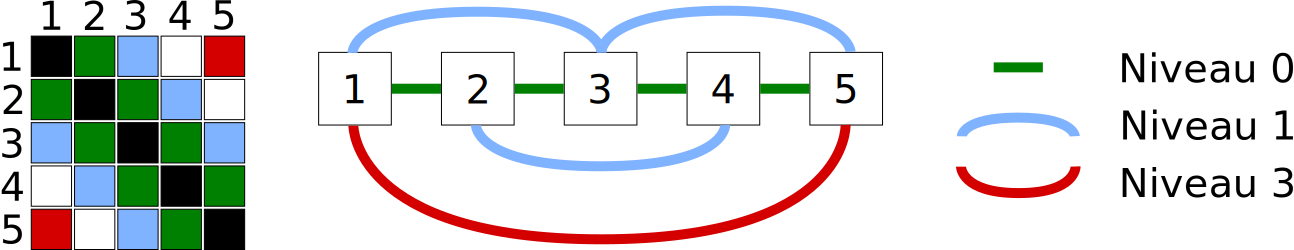
\includegraphics[width=0.9\linewidth]{iluk_filling}}

\end{frame}


%-------------------------------
\begin{frame}
  \frametitle{Vue hiérarchique d'une grappe de serveur}

  \centerline{\includegraphics[width=\linewidth]{cluster}}
\end{frame}


%-------------------------------
\begin{frame}
  \frametitle{Machine NUMA}
  \centerline{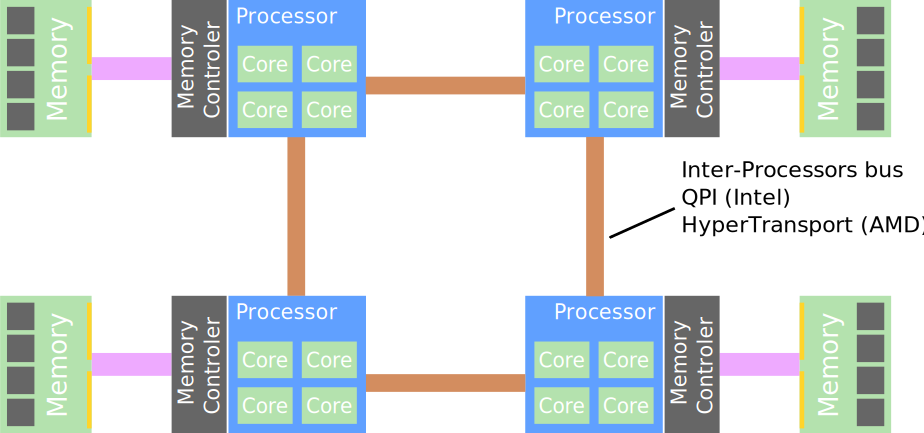
\includegraphics[width=0.8\linewidth]{numa}}

  \begin{itemize}
    \item Séparation physique de la mémoire
    \item Temps de latence des accès mémoire variable
  \end{itemize}

\end{frame}




%-------------------------------
\begin{frame}
  \frametitle{Programmation parallèle - Mémoire distribuée}
  Exemple : MPI
  \bigskip

  Avantages :
  \begin{itemize}
    \item Permet l'utilisation de plusieurs noeuds de calcul
    \item Utilisation de machines hétérogènes
  \end{itemize}

  Inconvénients :
  \begin{itemize}
    \item Certains algorithmes ne peuvent pas être paralléliser
  \end{itemize}

  \bigskip
  Problème de passage à l'échelle de certains algorithmes que nous utilisons (AMG).
\end{frame}



%-------------------------------
\begin{frame}
  \frametitle{Programmation parallèle - Parallélisme de boucle}
  Exemple : OpenMP
  \bigskip

  Avantages :
  \begin{itemize}
    \item Peu coûteux en temps de développement
    \item Utilisation de la mémoire partagée
  \end{itemize}

  Inconvénients :
  \begin{itemize}
    \item Limitations dans la description du parallélisme
  \end{itemize}

  \bigskip
  Ne permet pas de décrire le parallélisme d'une factorisation ILU.
\end{frame}



%-------------------------------
\begin{frame}
  \frametitle{Programmation parallèle - Tâches}
  Exemple : Cilk, Intel TBB, OpenMP3
  \bigskip

  Avantages :
  \begin{itemize}
    \item Description exhaustif du parallélisme
    \item Utilisation de la mémoire partagée
    \item Possibilité de l'utiliser en mémoire distribuée
  \end{itemize}

  Inconvénients :
  \begin{itemize}
    \item Complexe à utiliser (par rapport au parallélisme de boucle)
  \end{itemize}
\end{frame}

%-------------------------------
%-------------------------------
  \begin{frame}<beamer>
    \frametitle{Plan}
    \tableofcontents
  \end{frame}
%-------------------------------
%-------------------------------

%-------------------------------
\begin{frame}[fragile]
  \frametitle{Exemple de graphe de tâches}


\begin{lstlisting}
a = fun1(0);
b = fun2(a);
c = fun3(a);
d = fun4(b, c);
\end{lstlisting}

  \centerline{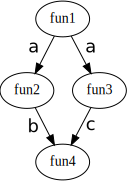
\includegraphics[width=0.25\linewidth]{agg_exemple}}
\end{frame}


%-------------------------------
\begin{frame}
  \frametitle{Programmation par graphe de tâches}

  \centerline{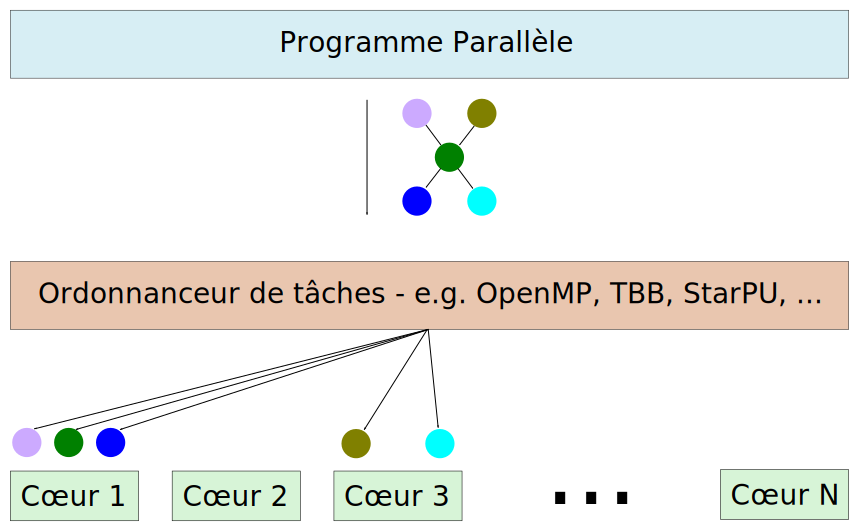
\includegraphics[width=0.8\linewidth]{runtime}}

  Principes de la programmation par graphe de tâches :
  \begin{itemize}
    \item Une tâche correspond à une portion de code
    \item Les tâches sont relié entre elles par des dépendances
    \item Besoin d'un ordonnanceur (efficace) de tâches
  \end{itemize}
\end{frame}


%-------------------------------
\begin{frame}
  \frametitle{Intergiciels à base de raphes de tâches - StarPU}

  \centerline{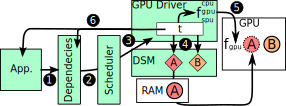
\includegraphics[width=0.7\linewidth]{starpu}}

  Caractéristiques :
  \begin{itemize}
    \item Architectures hétérogènes (CPU+GPU)
    \item Gestion transparente des transferts mémoire (DSM)
    \item Stratégies d'ordonnancement (dmda, eager ...)
    \item Description dynamique du graphe (insert-task)
  \end{itemize}

\end{frame}


%-------------------------------
\begin{frame}
  \frametitle{Intergiciels à base de graphes de tâches - PaRSEC}

  \centerline{\includegraphics[width=0.8\linewidth]{parsec}}

  Caractéristiques :
  \begin{itemize}
    \item Graphe de tâches paramétré (PTG)
    \item Gestion de la mémoire distribuée
    \item Utilisation du même graphe en mémoire distribuée et en mémoire partagée
    \item Support des architectures NUMA
  \end{itemize}
\end{frame}

%-------------------------------
\begin{frame}
  \frametitle{Propriétés des graphes de tâches}


  \centerline{\includegraphics[width=0.8\linewidth]{graphe_exemple}}


  Largeur du graphe $\approx$ Parallélisme


  Hauteur du graphe $\approx$ Temps d'exécution avec un parallélisme infini
\end{frame}


%-------------------------------
\begin{frame}
  \frametitle{Factorisation ILU(0)}

  \begin{itemize}
    \item Préconditionneur pour GMRES
  \end{itemize}

\begin{algorithm}[H]
\begin{algorithmic}[1]
  \STATE $M$ : matrice de dimension $n$
  \FOR{$i = 2$ \TO $n$}
  \STATE{\FOR{$k = 1$ \TO $i - 1$ \AND $M_{ik} != 0$}
    \STATE{$M_{ik} = M_{ik} / M_{kk}$
      \FOR{$j = k + 1$ \TO $n$ \AND $M_{ij} != 0$}
      \STATE{$M_{ij} = M_{ij} - M_{ik}M_{kj}$}
      \ENDFOR}
    \ENDFOR}
  \ENDFOR
\end{algorithmic}
\end{algorithm}

\end{frame}


%-------------------------------
\begin{frame}
  \frametitle{Factorisation ILU(0) - Graphe de tâches}

  \begin{itemize}
    \item Factorisation d'une ligne de la matrice par tâche
    \item Description naturelle du parallélisme
  \end{itemize}

  \centerline{\includegraphics[width=\linewidth]{G1}}
\end{frame}




%-------------------------------
\begin{frame}
  \frametitle{Factorisation ILU(0) - Premiers résultats}

  \begin{itemize}
        \item Plus d'un million de tâches
        \item 1 tâche dure en moyenne $100\,ns$
        \item La gestion d'une tâche coûte environ $500\,ns$
  \end{itemize}

  \begin{alertblock}{Problème}
    ILU(0) est seulement 2 fois plus rapide sur 12 coeurs que la version séquentielle.
  \end{alertblock}
  \pause
  Temps d'exécution d'un graphe de tâches :

  \bigskip

  $\frac{\sum Temps\_tache + \sum Temps\_Repos + nombre\_de\_taches * surcout}{nombre\_de\_coeurs}$
\end{frame}

%-------------------------------
\begin{frame}
  \frametitle{Effet de bord de la parallélisation par graphe de tâches}

  De plus :
  \begin{itemize}
    \item L'ordre de factorisation des lignes de la matrice impact les performances
    \item Les tâches ont des affinités entre elles (effet de cache)
  \end{itemize}

  \centerline{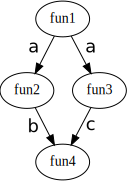
\includegraphics[width=0.15\linewidth]{agg_exemple}}

  Exemple pour ILU(0) sur une matrice d'un million de lignes :
  \begin{itemize}
    \item Factorisation des lignes avec un parcourt linéaire : 0,43~s
    \item Factorisation des lignes avec un parcourt non-linéaire : 1,43~s
  \end{itemize}


\end{frame}



%-------------------------------
\begin{frame}
  \frametitle{Granularité des tâches de calcul}

  Temps d'exécution d'un graphe de tâches :

  \bigskip

  $\frac{\sum Temps\_tache(tache\_precedente) + \sum Temps\_Repos + nombre\_de\_taches * surcout}{nombre\_de\_coeurs}$

  \pause

  \begin{itemize}
  \item<2-> La granularité dépend du rapport entre le surcout d'ordonnancement et le temps d'exécution des tâches
  \item<2-> On souhaite avoir un surcout plusieurs fois plus petit que le temps d'exécution des tâches
  \item<2-> Or, dans notre cas, ce surcout est plus grand
  \end{itemize}

  \pause

  \begin{block}{Solution}
    Diminuer le nombre de tâche, conserver suffisament de parallélisme et exécuter les tâches dans le meilleur ordre possible.
  \end{block}


\end{frame}

%=========================================================
\section{Heuristiques d'agrégation}
%=========================================================
%-------------------------------
\begin{frame}
  \frametitle{Diminuer le nombre de tâches}

  \centerline{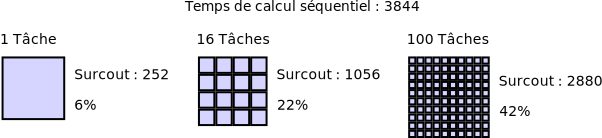
\includegraphics[width=\linewidth]{overhead}}


  \begin{itemize}
    \item Exécuter le travail de plusieurs tâches dans une tâche
    \item Conserver assez de parallélisme
  \end{itemize}

\end{frame}


%-------------------------------
\begin{frame}[fragile]
  \frametitle{Problème du cycle}

\begin{lstlisting}
a = fun1(0);
b = fun2(a);
c = fun3(a);
d = fun4(b, c);
\end{lstlisting}

  \centerline{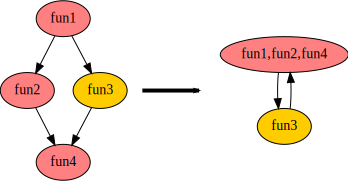
\includegraphics[width=0.8\linewidth]{agg_invalid}}
\end{frame}


%-------------------------------
\begin{frame}
  \frametitle{Largeur et hauteur du graphe}

  \begin{itemize}
    \item Ne pas trop diminuer la largeur
  \end{itemize}

  \centerline{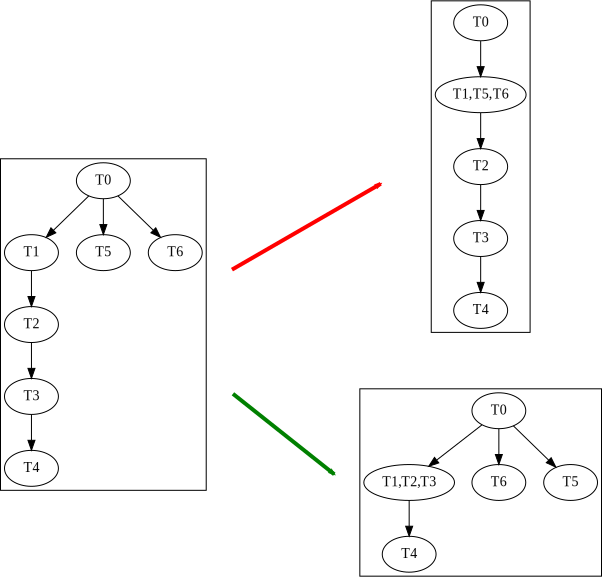
\includegraphics[width=0.6\linewidth]{agg_hl}}
\end{frame}


%-------------------------------
\begin{frame}
  \frametitle{Agréger des tâches}

  Changement des propriétés du graphe :
  \begin{itemize}
    \item Graphe acyclique
    \item Largeur du graphe
    \item Hauteur du graphe
    \item Affinités entre les tâches
  \end{itemize}

\end{frame}

%-------------------------------
\begin{frame}
  \frametitle{Taggre}

  \centerline{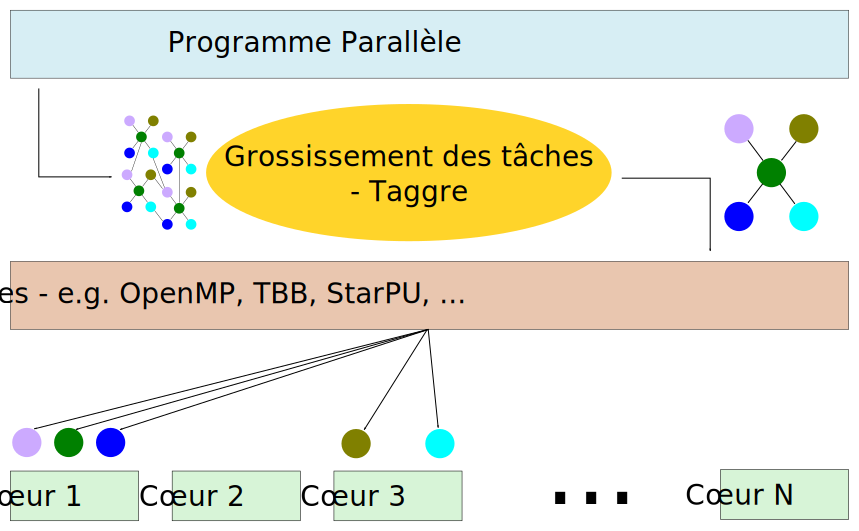
\includegraphics[width=0.55\linewidth]{coarsening}}

  \begin{itemize}
    \item \'Etape supplémentaire entre la description du graphe de tâches et l'exécution de celui-ci
    \item Permet d'augmenter la granularité en groupant dans tâches entre elles
  \end{itemize}

  \begin{block}{Grossissement des tâches}
    \`A partir d'un graphe à grain fin, on calcul un graphe plus grossier en appliquant
    des heuristiques de grossissement.
  \end{block}
\end{frame}


%-------------------------------
\begin{frame}
  \frametitle{Taggre - Heuristique d'agrégation}

  \centerline{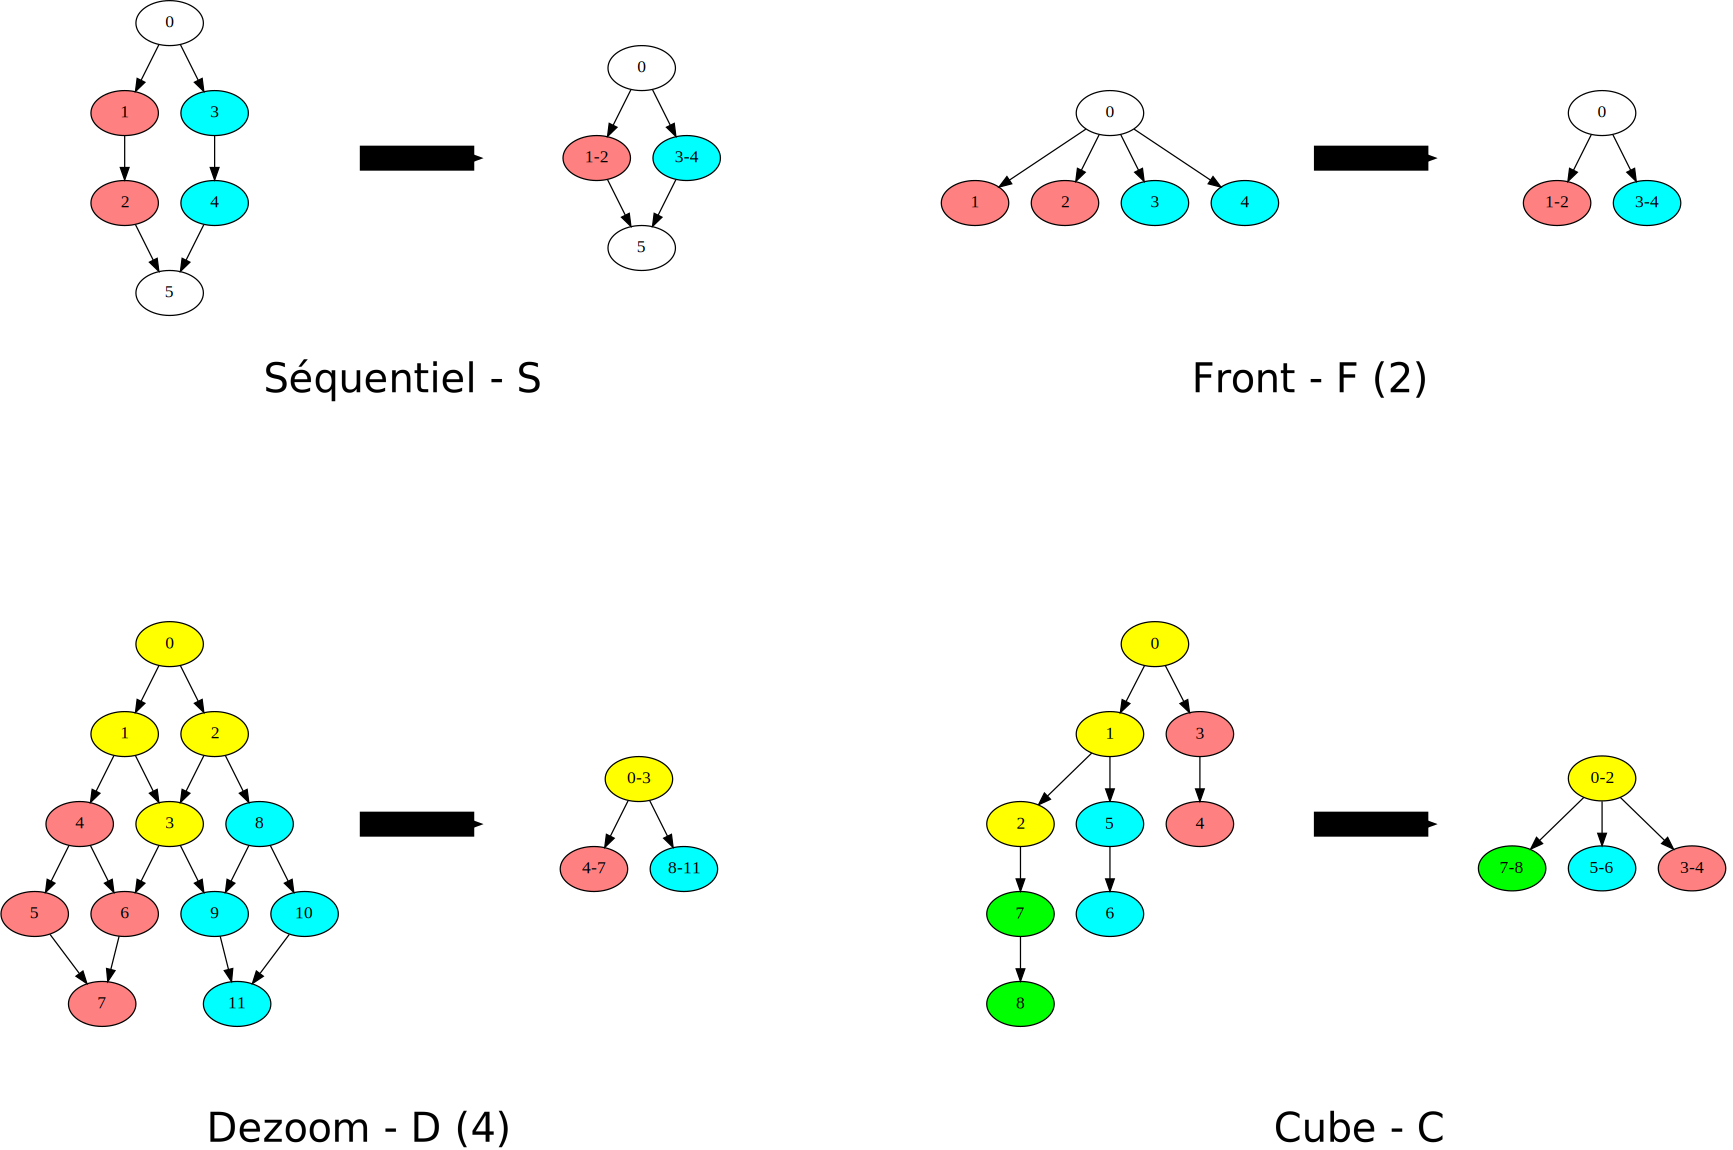
\includegraphics[width=0.80\linewidth]{all_algo}}

  \begin{itemize}
    \item 4 heuristiques pour modifier le graphe
    \item Certaines heuristiques prennent un paramètre en entrée
    \item Chaque heuristique aura un avantage spécifique
  \end{itemize}
\end{frame}



%-------------------------------
\begin{frame}
  \frametitle{Séquentiel (S)}

  \centerline{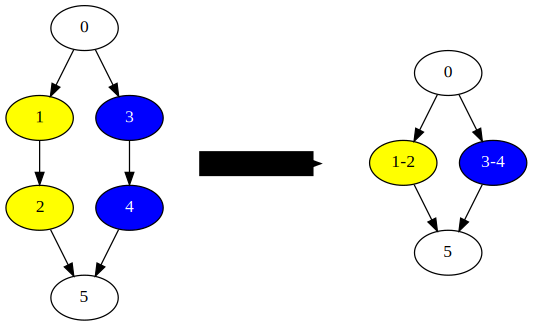
\includegraphics[width=0.80\linewidth]{algo_S}}

  \begin{block}{Objectif}
    Réduire la hauteur du graphe sans impacter le parallélisme.
  \end{block}
\end{frame}



%-------------------------------
\begin{frame}
  \frametitle{Front (F)}

  \centerline{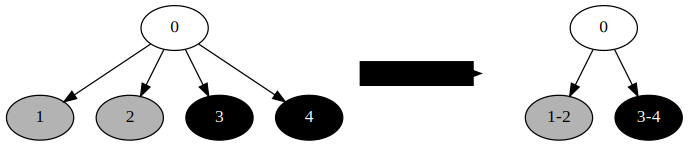
\includegraphics[width=0.80\linewidth]{algo_F2}}

  \bigskip
  \bigskip

  Prend en paramètre la largeur du graphe souhaitée.

  \bigskip

  \begin{block}{Objectif}
    Réduire le parallélisme superflu.
  \end{block}
\end{frame}


%-------------------------------
\begin{frame}
  \frametitle{Cube (C)}

  \centerline{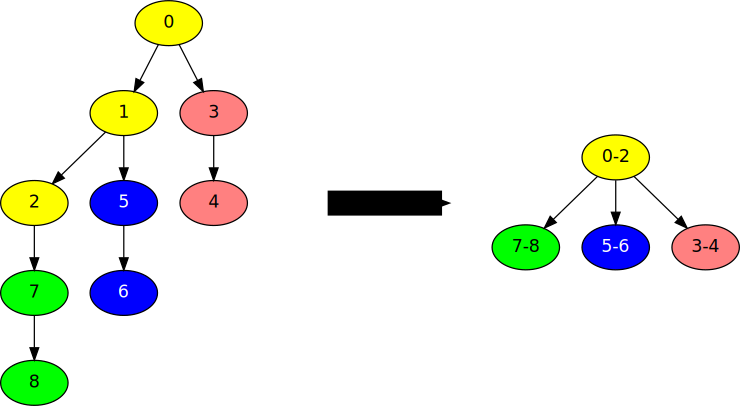
\includegraphics[width=0.80\linewidth]{algo_3}}

  \begin{block}{Objectif}
    Favoriser les effets de cache sur les modèles structurés.
  \end{block}
\end{frame}



%-------------------------------
\begin{frame}
  \frametitle{Dezoom (D)}

  \centerline{\includegraphics[width=0.75\linewidth]{algo_D4}}

  \bigskip

  Prend en paramètre le nombre de tâches par groupe de tâche.

  \bigskip

  \begin{block}{Objectif}
    Créer des groupes de tâches spatialement proches.
  \end{block}
\end{frame}


%-------------------------------
\begin{frame}
  \frametitle{Dezoom (D)}

  \begin{itemize}
    \item Simuler l'exécution pour éviter les cycles.
    \item Utilisation d'une fonction d'évaluation pour connaître la prochaine tâche à agréger :
    \begin{itemize}
      \item Prise en compte de la distance aux autres tâches
      \item Prise en compte du nombre de dépendances
      \item Possibilité de privilégier la hauteur ou la largeur
    \end{itemize}
  \end{itemize}

  \centerline{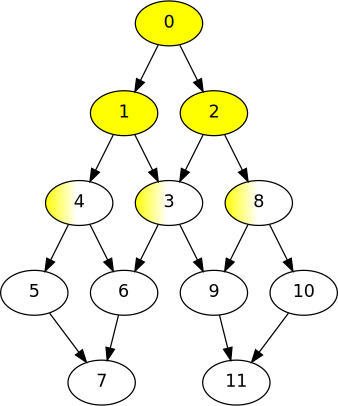
\includegraphics[width=0.35\linewidth]{algo_D_ongoing}}

\end{frame}



%-------------------------------
\begin{frame}
  \frametitle{Synthèse autour de Taggre}

  \begin{itemize}
    \item Le programmeur doit choisir les algorithmes à appliqués
    \item Possibilité de chaîner les heuristiques
    \item Le choix des paramètres des heuristiques n'est pas difficile :
      \begin{itemize}
        \item D dépend de la granularité du problème
        \item F dépend du nombre de coeurs de la machine
      \end{itemize}
    \item F s'utilisera toujours en dernier
    \item C s'utilisera en premier si le cas le permet
    \item \'Etape plus simple que de réécrire le programme avec une granularité différente
    \item Possibilité de sauvegarder les agrégations
  \end{itemize}

\end{frame}


%=========================================================
\section{Application à ILU(0)}
%=========================================================
%-------------------------------
\begin{frame}[fragile,allowframebreaks]
  \frametitle{Exemple de code}

 \begin{lstlisting}
/* Creer l'objet graphe */
Schema schema("Graph_Name");

/* Creer les taches */
vector<int> my_tasks;
for (int i = 0; i < nb_rows; i++)
 my_tasks.push_back(schema.new_task(1, i));

/* Declarer les dependances */
for (int i = 0; i < nb_rows; i++)
 for (int j = 0; j < diag[i]; j++)
  schema.declare_dependency(my_tasks[j],my_tasks[i])
 \end{lstlisting}


\framebreak

 \begin{lstlisting}
/* Grossissement du graphe */
schema.coarse("CF(4)");

/* Creer les taches utilisateurs */
schema.setup([](int n, int *ids, int *weights,
                int *affinities, void **tasks_info) -> Task* {
  return new my_class(n, affinities);
});
 \end{lstlisting}
\framebreak

 \begin{lstlisting}

/* Utilisation de la methode execute de chaque tache */
schema.run();

/* Utilisation d'une autre fonction */
schema.run([&](Task *t)
  {
    compute((my_class*)t);
  });
 \end{lstlisting}

\end{frame}

%-------------------------------
\begin{frame}
  \frametitle{}
  \centerline{\includegraphics[width=0.9\linewidth]{G_agg}}
\end{frame}

%-------------------------------
\begin{frame}
  \frametitle{Protocole de test}
  Machine :
  \begin{itemize}
    \item 2 processeurs Intel Xeon X5660
    \item 6 coeurs de calcul par processeur
    \item 48~Go de mémoire vive
    \item 2 bancs NUMA
  \end{itemize}

  Cas test :
  \begin{itemize}
    \item Matrice d'un million de lignes
    \item 7 diagonales
    \item Chaque entrée de la matrice est un bloc 3x3
  \end{itemize}

  Moyenne des 5 résultats médians sur 10 lancements.

\end{frame}

%-------------------------------
\begin{frame}
  \frametitle{Résultat - ILU(0) - 12 coeurs}
  \centerline{\includegraphics[width=0.8\linewidth]{res_ilu0}}
\end{frame}


%-------------------------------
\begin{frame}
  \frametitle{Résultat - ILU(2) - 12 coeurs}
  \centerline{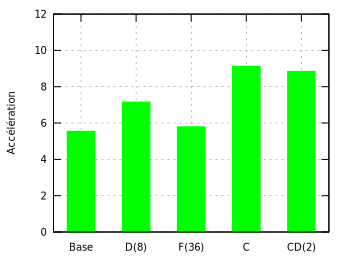
\includegraphics[width=0.8\linewidth]{res_iluk}}
\end{frame}


%-------------------------------
\begin{frame}
  \frametitle{Problèmes restants}

  Surcout d'agrégation :
  \begin{itemize}
    \item L'étape d'agrégation coûte du temps (environ 2~s pour notre cas test)
    \item Possibilité de l'amortir en utilisant plusieurs fois le graphe ($\approx$10)
    \item En algèbre linéaire creuse, ce graphe est réutilisé plusieurs fois
  \end{itemize}

  Mémoire :
  \begin{itemize}
    \item Performances de l'algorithme ILU(k) limitées par la bande passante mémoire
    \item Utilisation incomplète de la bande passante mémoire des machines NUMA
  \end{itemize}
\end{frame}

%=========================================================
\section[Aspects NUMA]{Prise en compte des aspects NUMA dans la gestion des données}
%=========================================================
%-------------------------------
\begin{frame}
  \frametitle{Produit matrice-vecteur creux}
  \centerline{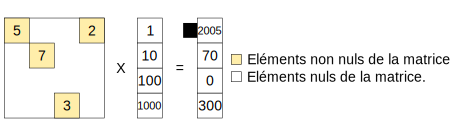
\includegraphics[width=\linewidth]{spmv}}

  \begin{itemize}
    \item Parallélisme de boucle
    \item Accélération de 2 sur 12 coeurs de calcul
    \item Peu de réutilisation des caches
    \item Limitation liée à la mémoire
  \end{itemize}
\end{frame}


%-------------------------------
\begin{frame}
  \frametitle{Le modèle roofline}
  \centerline{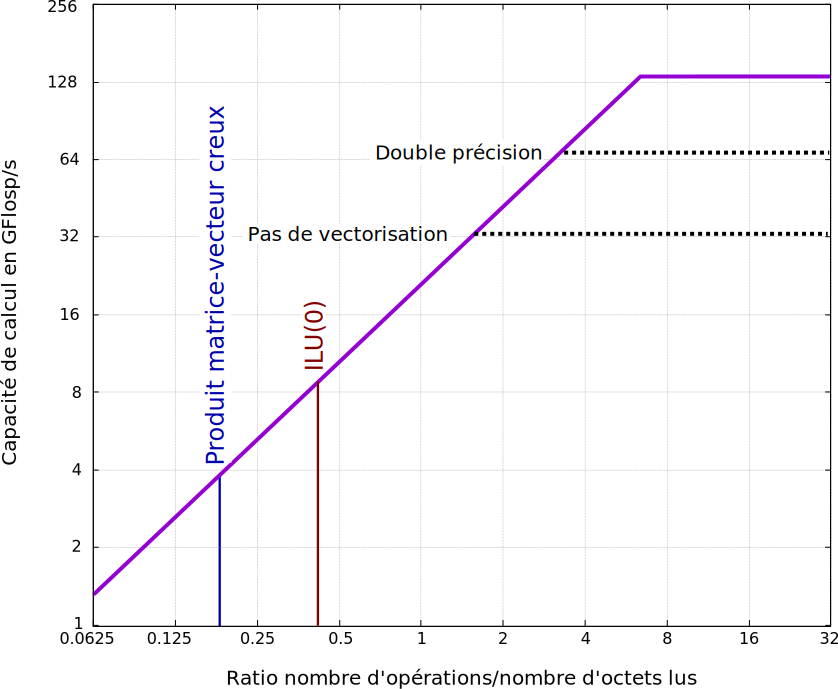
\includegraphics[width=0.8\linewidth]{roofline_rostand}}
\end{frame}


%-------------------------------
\begin{frame}
  \frametitle{Machine NUMA}
  \centerline{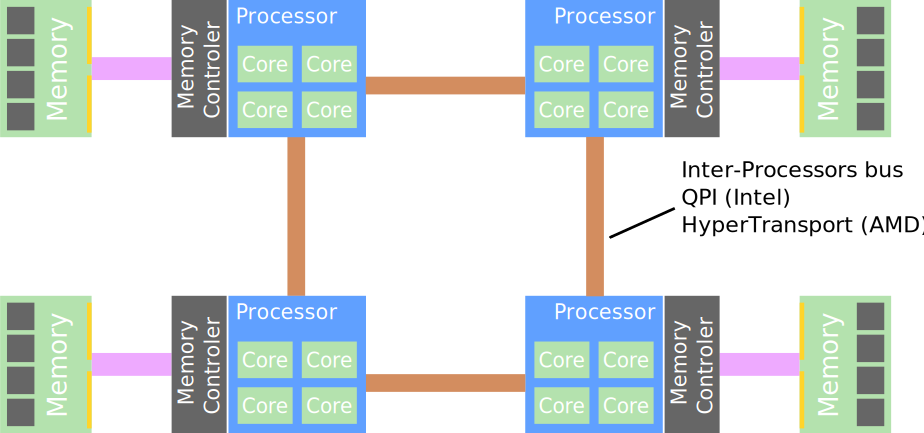
\includegraphics[width=0.8\linewidth]{numa}}

  \begin{itemize}
    \item Réduction de la contention sur le controleur mémoire par rapport à SMP
    \item Gestion plus difficile des allocations mémoire
  \end{itemize}

\end{frame}

%-------------------------------
\begin{frame}
  \frametitle{Gestion mémoire virtuelle}
  \centerline{\includegraphics[width=0.8\linewidth]{virtual}}

  \begin{itemize}
    \item Les processus ne voient qu'un espace d'adressage virtuel
    \item Le noyau s'occupe d'assigner une adresse physique à une adresse virtuelle
    \item Migration physique transparente
  \end{itemize}
\end{frame}

%-------------------------------
\begin{frame}
  \frametitle{Stratégies d'allocation mémoire I}

  \begin{block}{First touch}
    Allocation de la mémoire au plus proche du coeur qui l'utilise en premier.
  \end{block}

  \pause

  \begin{block}{Interleave}
    Allocation en mode tourniquet.
  \end{block}

  \pause

  \begin{block}{Bind}
    Le programmeur choisi l'emplacement des données.
  \end{block}
\end{frame}


%-------------------------------
\begin{frame}
  \frametitle{Stratégies d'allocation mémoire II}

  \begin{block}{Next-touch}
    Migration des données déjà allouées lors du prochain accès.
  \end{block}

  \pause

  \begin{block}{AutoNUMA (Linux 3.13+)}
    \'Equilibrage automatique pendant l'exécution du programme.
  \end{block}

  \pause

  \begin{block}{Bibliothèques externes}
    Bibliothèques fournissant des stratégies d'allocations et de migrations mémoire (MaMI, MAi ...)
  \end{block}

\end{frame}


%-------------------------------
\begin{frame}
  \frametitle{Couplage à un ordonnanceur de tâches}

  \begin{itemize}
    \item Lier des données aux tâches
    \item Exécuter les tâches sur coeur proche des données
    \item Migration physique des données pour améliorer la répartition de charge
  \end{itemize}

  \pause

  \begin{alertblock}{Ordonnanceur NUMA}
    Peu d'ordonnanceurs disponibles (PaRSEC, StarSs ...). Ils ne répondent pas à notre besoin.
  \end{alertblock}

\end{frame}



%-------------------------------
\begin{frame}
  \frametitle{NATaS}

  \begin{itemize}
    \item Possibilité de choisir l'affinité NUMA d'une tâche
    \item Ordonnanceur très simple
    \item Une structure de donnée par banc NUMA
  \end{itemize}

  \pause

  Couplage à Taggre :
  \begin{itemize}
    \item Les tâches d'un graphe sont distribuées par hauteur dans le graphe
    \item Migration des données pour faire correspondre à l'affinité NUMA des tâches
  \end{itemize}

\end{frame}

%-------------------------------
\begin{frame}
  \frametitle{Exemple de distribution d'un graphe}

  \centerline{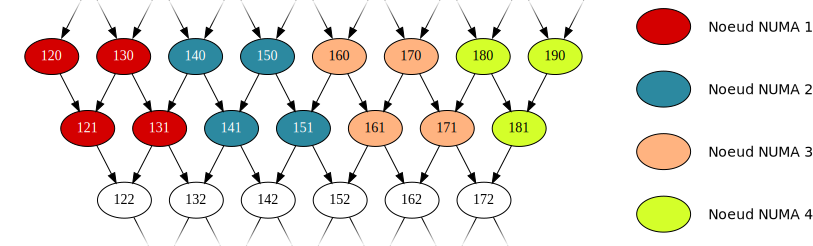
\includegraphics[width=\linewidth]{numa_distrib_example}}

\end{frame}


%-------------------------------
\begin{frame}
  \frametitle{Résultats du produit matrice-vecteur creux - 12 coeurs}

  \centerline{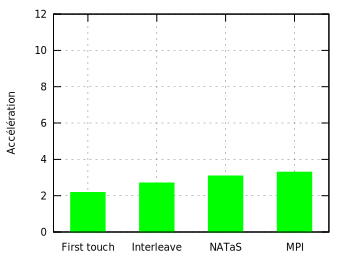
\includegraphics[width=0.8\linewidth]{res_ilu_spmv}}

\end{frame}

%-------------------------------
\begin{frame}
  \frametitle{Résultats de la factorisation ILU(0) - 12 coeurs}

  \centerline{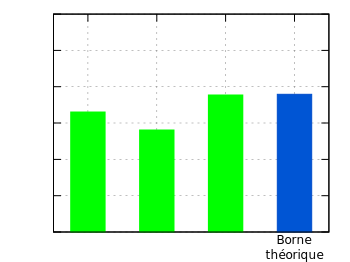
\includegraphics[width=0.8\linewidth]{res_ilu_nas}}

\end{frame}

%-------------------------------
\begin{frame}
  \frametitle{Résultats de la factorisation ILU(0) - 160 coeurs - 20 bancs NUMA}

  \centerline{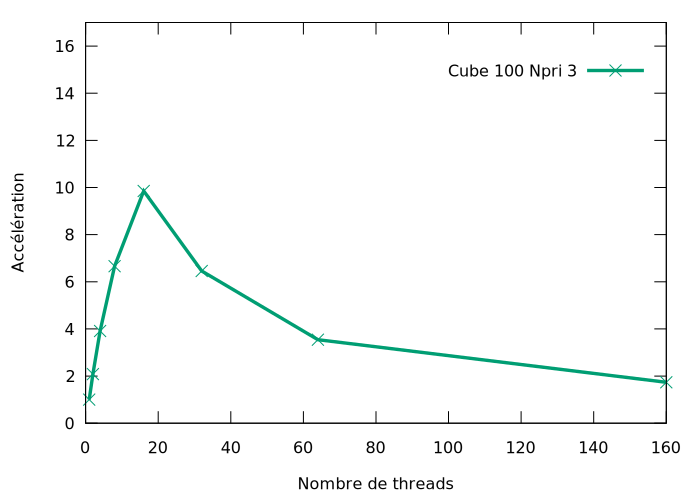
\includegraphics[width=0.8\linewidth]{manumanu}}

\end{frame}


%=========================================================
\section{Conclusion et perspectives}
%=========================================================
%-------------------------------
\begin{frame}
  \frametitle{Conclusion et perspectives}
         Conclusion :
    \begin{itemize}
      \item<1-> Nouvel outils générique pour grossir le grain d'un graphe
      \item<1-> Amélioration de la parallélisation de noyaux d'algèbre linéaire creuse (ILU, TRSV, SpMV ...)
      \item<1-> Meilleure utilisation de la bande passante mémoire
    \end{itemize}
    \pause

         \bigskip
         \bigskip

    Perspectives :
    \begin{itemize}
      \item<2-> Automatiser les paramètres des opérateurs d'agrégation
      \item<2-> \'Etendre NATaS pour les machines composées de nombreux bancs NUMA
      \item<2-> Fusionner les graphes de tâches
    \end{itemize}
\end{frame}


%-------------------------------
\begin{frame}
  \frametitle{Fusion des graphes de tâches}

  \centerline{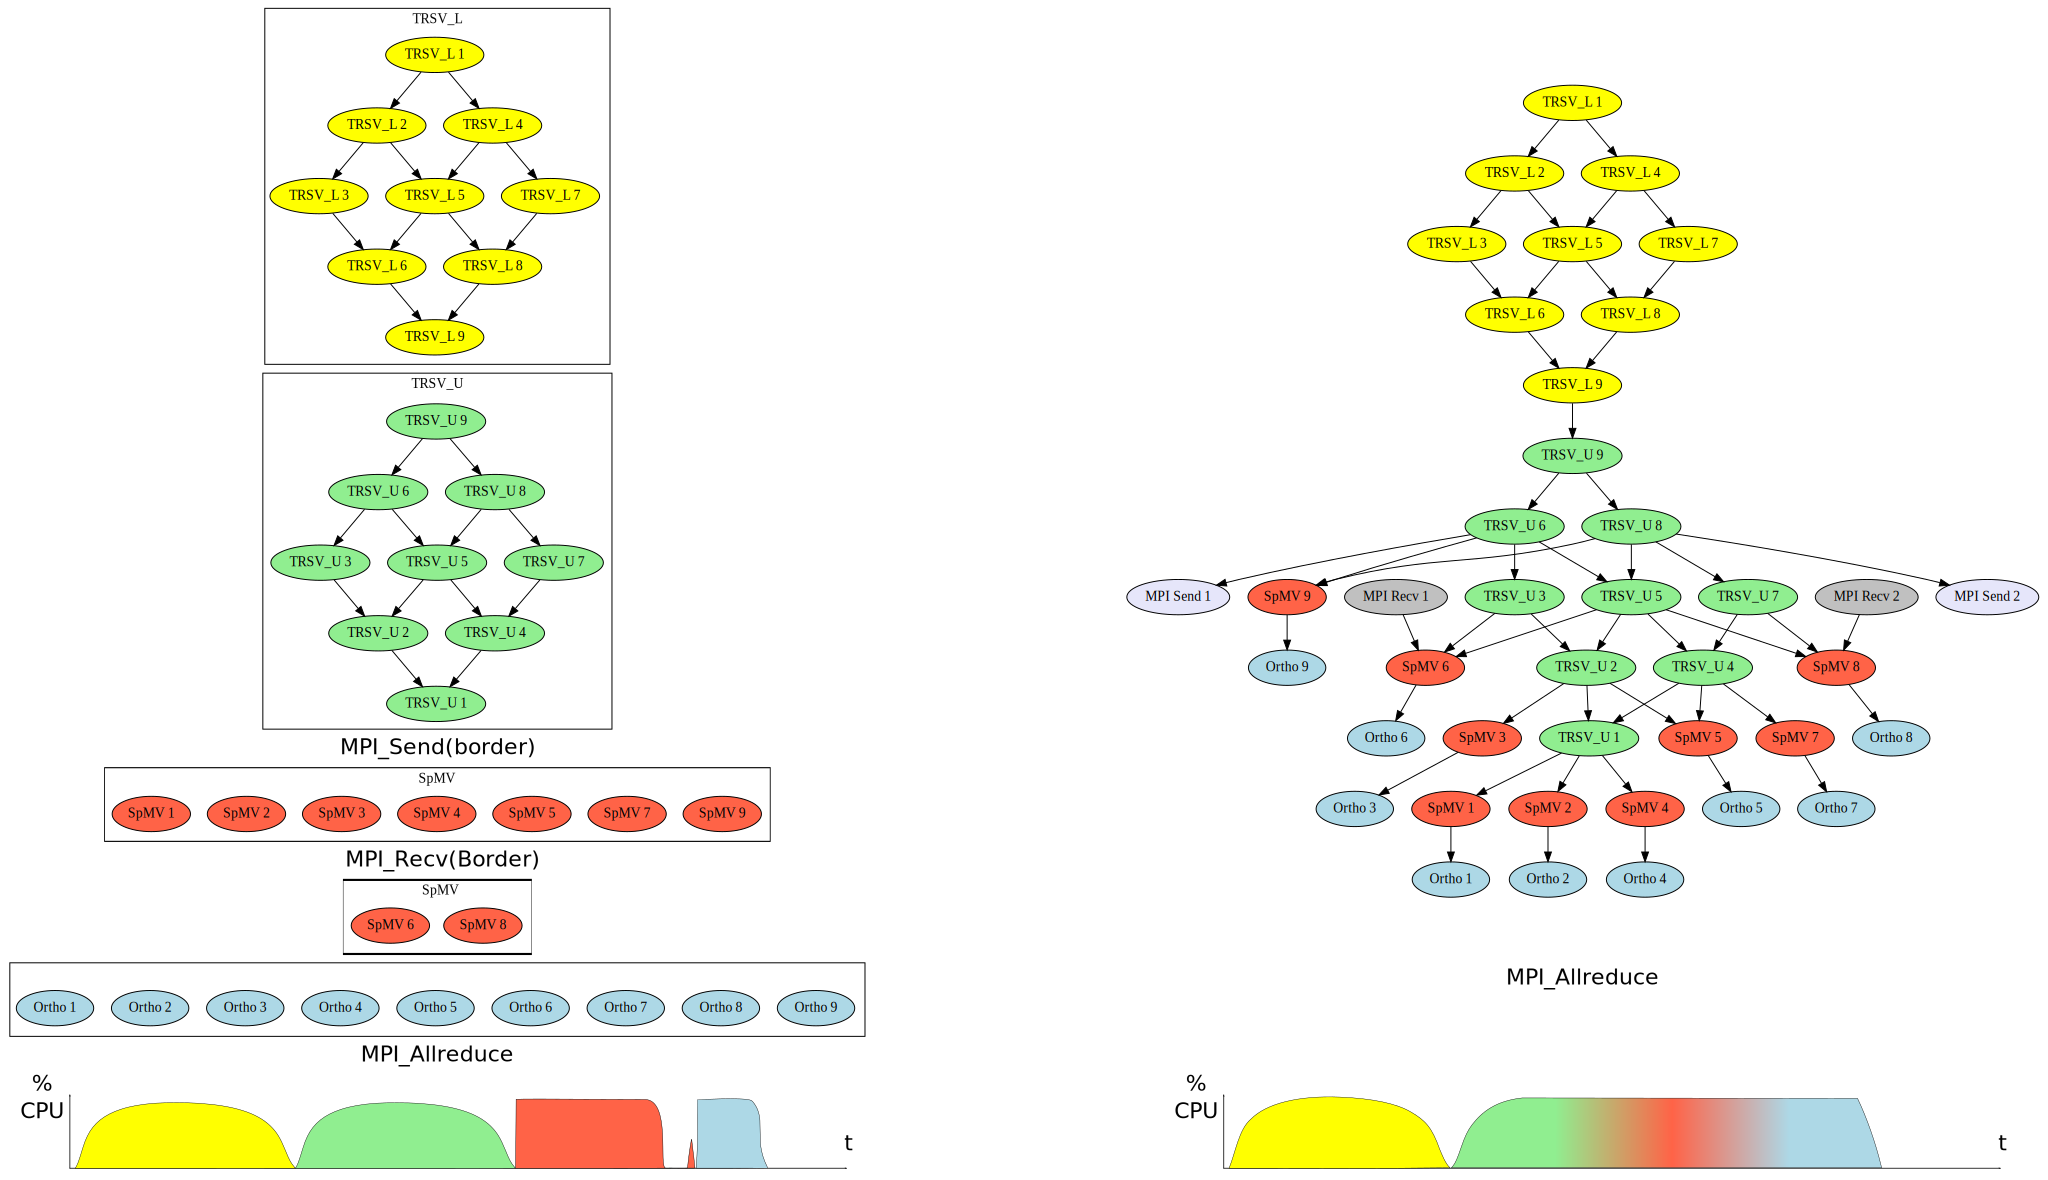
\includegraphics[width=\linewidth]{fusion}}
\end{frame}



%-------------------------------
\begin{frame}
  \frametitle{Questions}
  \begin{center}
    Merci de votre attention


         \bigskip
         \bigskip


   Avez-vous des questions ?
  \end{center}
\end{frame}


%=========================================================
%=========================================================
\backupbegin
%-------------------------------
\begin{frame}
  \frametitle{Résultats de la factorisation ILU(0) - AutoNUMA}

  \centerline{\includegraphics[width=0.8\linewidth]{autonuma}}

\end{frame}
\backupend



\end{document}
